% === [ Literature Review ] ====================================================

% <howto>
% * Critical review of relevant literature
%    - Not just what others have said, but also critique and reflect

% <howto> Doing a literature review
% * Define the problem
% * Literature search
% * Literature review
%    - Read and evaluate the literature
%    - Critically analyse what you have found
% * More than one iteration (continue throughout the project)

% <howto> suggested review approaches
% * Thematic
%    - explain about area of study: general review of area, concentrating on
%      academic literature
% * More focused
%    - e.g. some recent developments in the field
% * Chronological
%    - how the topic has evolved (but beware palaeontology)
% * Alternative theories and methods and explanation why they are relevant
% * SHORT overview of relevant tools

% <howto> literature search
% * Start broad, then focus
% * Redefine/refine search
%    - Continuous cycle: identify different thinking in the area

% <howto> marking notes
% * Uses credible, current material
% * Demonstrates understanding of complex subject and viewed in wider context
% * Shows originality and confidence in criticising assumptions
% * Well-justified critique of literature
% * Identifies flaws, gaps or inconsistencies in extant knowledge

% <howto>
% * What is the problem, or research question that my literature review helps to
%   define?
% * What is the scope of my literature review?
% * Has my search been wide enough to ensure I've found all the relevant
%   material and narrow enough to exclude irrelevant material?
% * Have I critically analysed the literature I use? Do I follow through a set
%   of concepts and questions, comparing items to each other in the ways they
%   deal with them? Instead of just listing and summarizing items, do I assess
%   them, discussing strengths and weaknesses?
% * IMPORTANT: Have I cited and discussed studies contrary to my perspective?

% <howto>
% * Write brief notes on each source (your own words, not their abstract):
%    - Key ideas (seminal sources, recognized theories)
%    - Novel ideas (proposed or demonstrated)
%    - Actual data (as distinct from mere argument)
%    - Outliers (contradict what everyone else says)
%    - Your critical evaluation: Is it convincing? Why? What are its
%      limitations? Is it current or out-of-date? What does it fail to address?

% <howto> common mistakes in writing a literature review
% * Writing your own opinion on a particular subject
% * Writing a list of summaries of sources , one after another, without
%   reviewing it
% * Writing an essay on everything you know about a particular subject

% <howto> What is a literature review?
% * A critical look at the published work relevant to your project
% * Gives the reader understanding of the problem area and the rationale for
%   what you are doing
% * What has already been done in your area
% * Sets the context for your project
% * Justifies your project

% <howto>
% * Main themes and key authors

% <howto>
% * a literature review is NOT an essay.
%    - NOT a detailed write up of a particular source.
%    - NOT just a summary of articles, texts or journals.
%    - NOT an opinionated or argumentative essay.
%
% --- [ essay ] ---
% * Use material to prove an argument or point of view, demonstrate
%   understanding.
% * Use relevant material.
% * Mentions authors/researchers only for reference.
%
% --- [ literature review ] ---
%
% * Critical analysis of material discovered about a subject.
% * Examine what has already been discovered.
% * Find patterns, gaps, conflicts.
% * Identify key researchers.
%
% * critical appraisal: the ability to apply principles of analysis to identify
%   unbiased and valid work.

% <howto>
% * What to notice when reading
%     - What is the line of reasoning?
%     - Is evidence presented? Does it stand up? (valid criteria)
%     - What do I think about it? Do I agree? Have I found supporting /
%       contradicting material?
%     - Are there assumptions / hidden agendas?
%     - What are the writer's conclusions? Does the evidence support them?
%     - Do not just select the parts of the literature that agree with what you
%       think

% <howto>
% * which authors support which views?
% * are there inconsistencies, gaps...?

\section{Literature Review}
\label{sec:literature_review}

This section details the problem domain associated with decompilation, reviews traditional decompilation techniques, and evaluates a set of intermediate representations with regards to their suitability for decompilation purposes. To set the stage for binary analysis, a \textit{``hello world''} executable is dissected in section~\ref{sec:lit_review_the_anatomy_of_an_executable}.

% === [ Subsections ] ==========================================================

% --- [ The Anatomy of an Executable ] -----------------------------------------

\subsection{The Anatomy of an Executable}
\label{sec:lit_review_the_anatomy_of_an_executable}

The representation of executables, shared libraries and relocatable object code is standardised by a variety of file formats which provides encapsulation of assembly instructions and data. Two such formats are the Portable Executable (PE) file format and the Executable and Linkable Format (ELF), which are used by Windows and Linux respectively. Both of these formats partition executable code and data into sections and assign appropriate access permissions to each section, as summarised by table \ref{tbl:elf_sections}. In general, no single section has both write and execute permissions as this could compromise the security of the system.

\begin{table}[htbp]
	\begin{center}
		\begin{tabular}{|l|l|l|}
			\hline
			Section name & Usage description & Access permissions \\
			\hline
			\texttt{.text} & Assembly instructions & \texttt{r-x} \\
			\texttt{.rodata} & Read-only data & \texttt{r--} \\
			\texttt{.data} & Data & \texttt{rw-} \\
			\texttt{.bss} & Uninitialised data & \texttt{rw-} \\
			\hline
		\end{tabular}
	\end{center}
	\caption{A summary of the most commonly used sections in ELF files. The \texttt{.text} section contains executable code while the \texttt{.rodata}, \texttt{.data} and \texttt{.bss} sections contains data in various forms.}
	\label{tbl:elf_sections}
\end{table}

To gain a better understanding of the anatomy of executables the remainder of this section describes the structure of ELF files and presents the dissection of a simple \textit{``hello world''} ELF executable, largely inspired by Eric Youngdale's article on \textit{The ELF Object File Format by Dissection} \cite{elf_by_dissection}. Although the ELF and PE file formats differ with regards to specific details, the general principles are applicable to both formats.

In general, ELF files consist of a file header, zero or more program headers, zero or more section headers and data referred to by the program or section headers, as depicted in figure \ref{fig:elf_file_structure}.

\begin{figure}[htbp]
	\begin{center}
		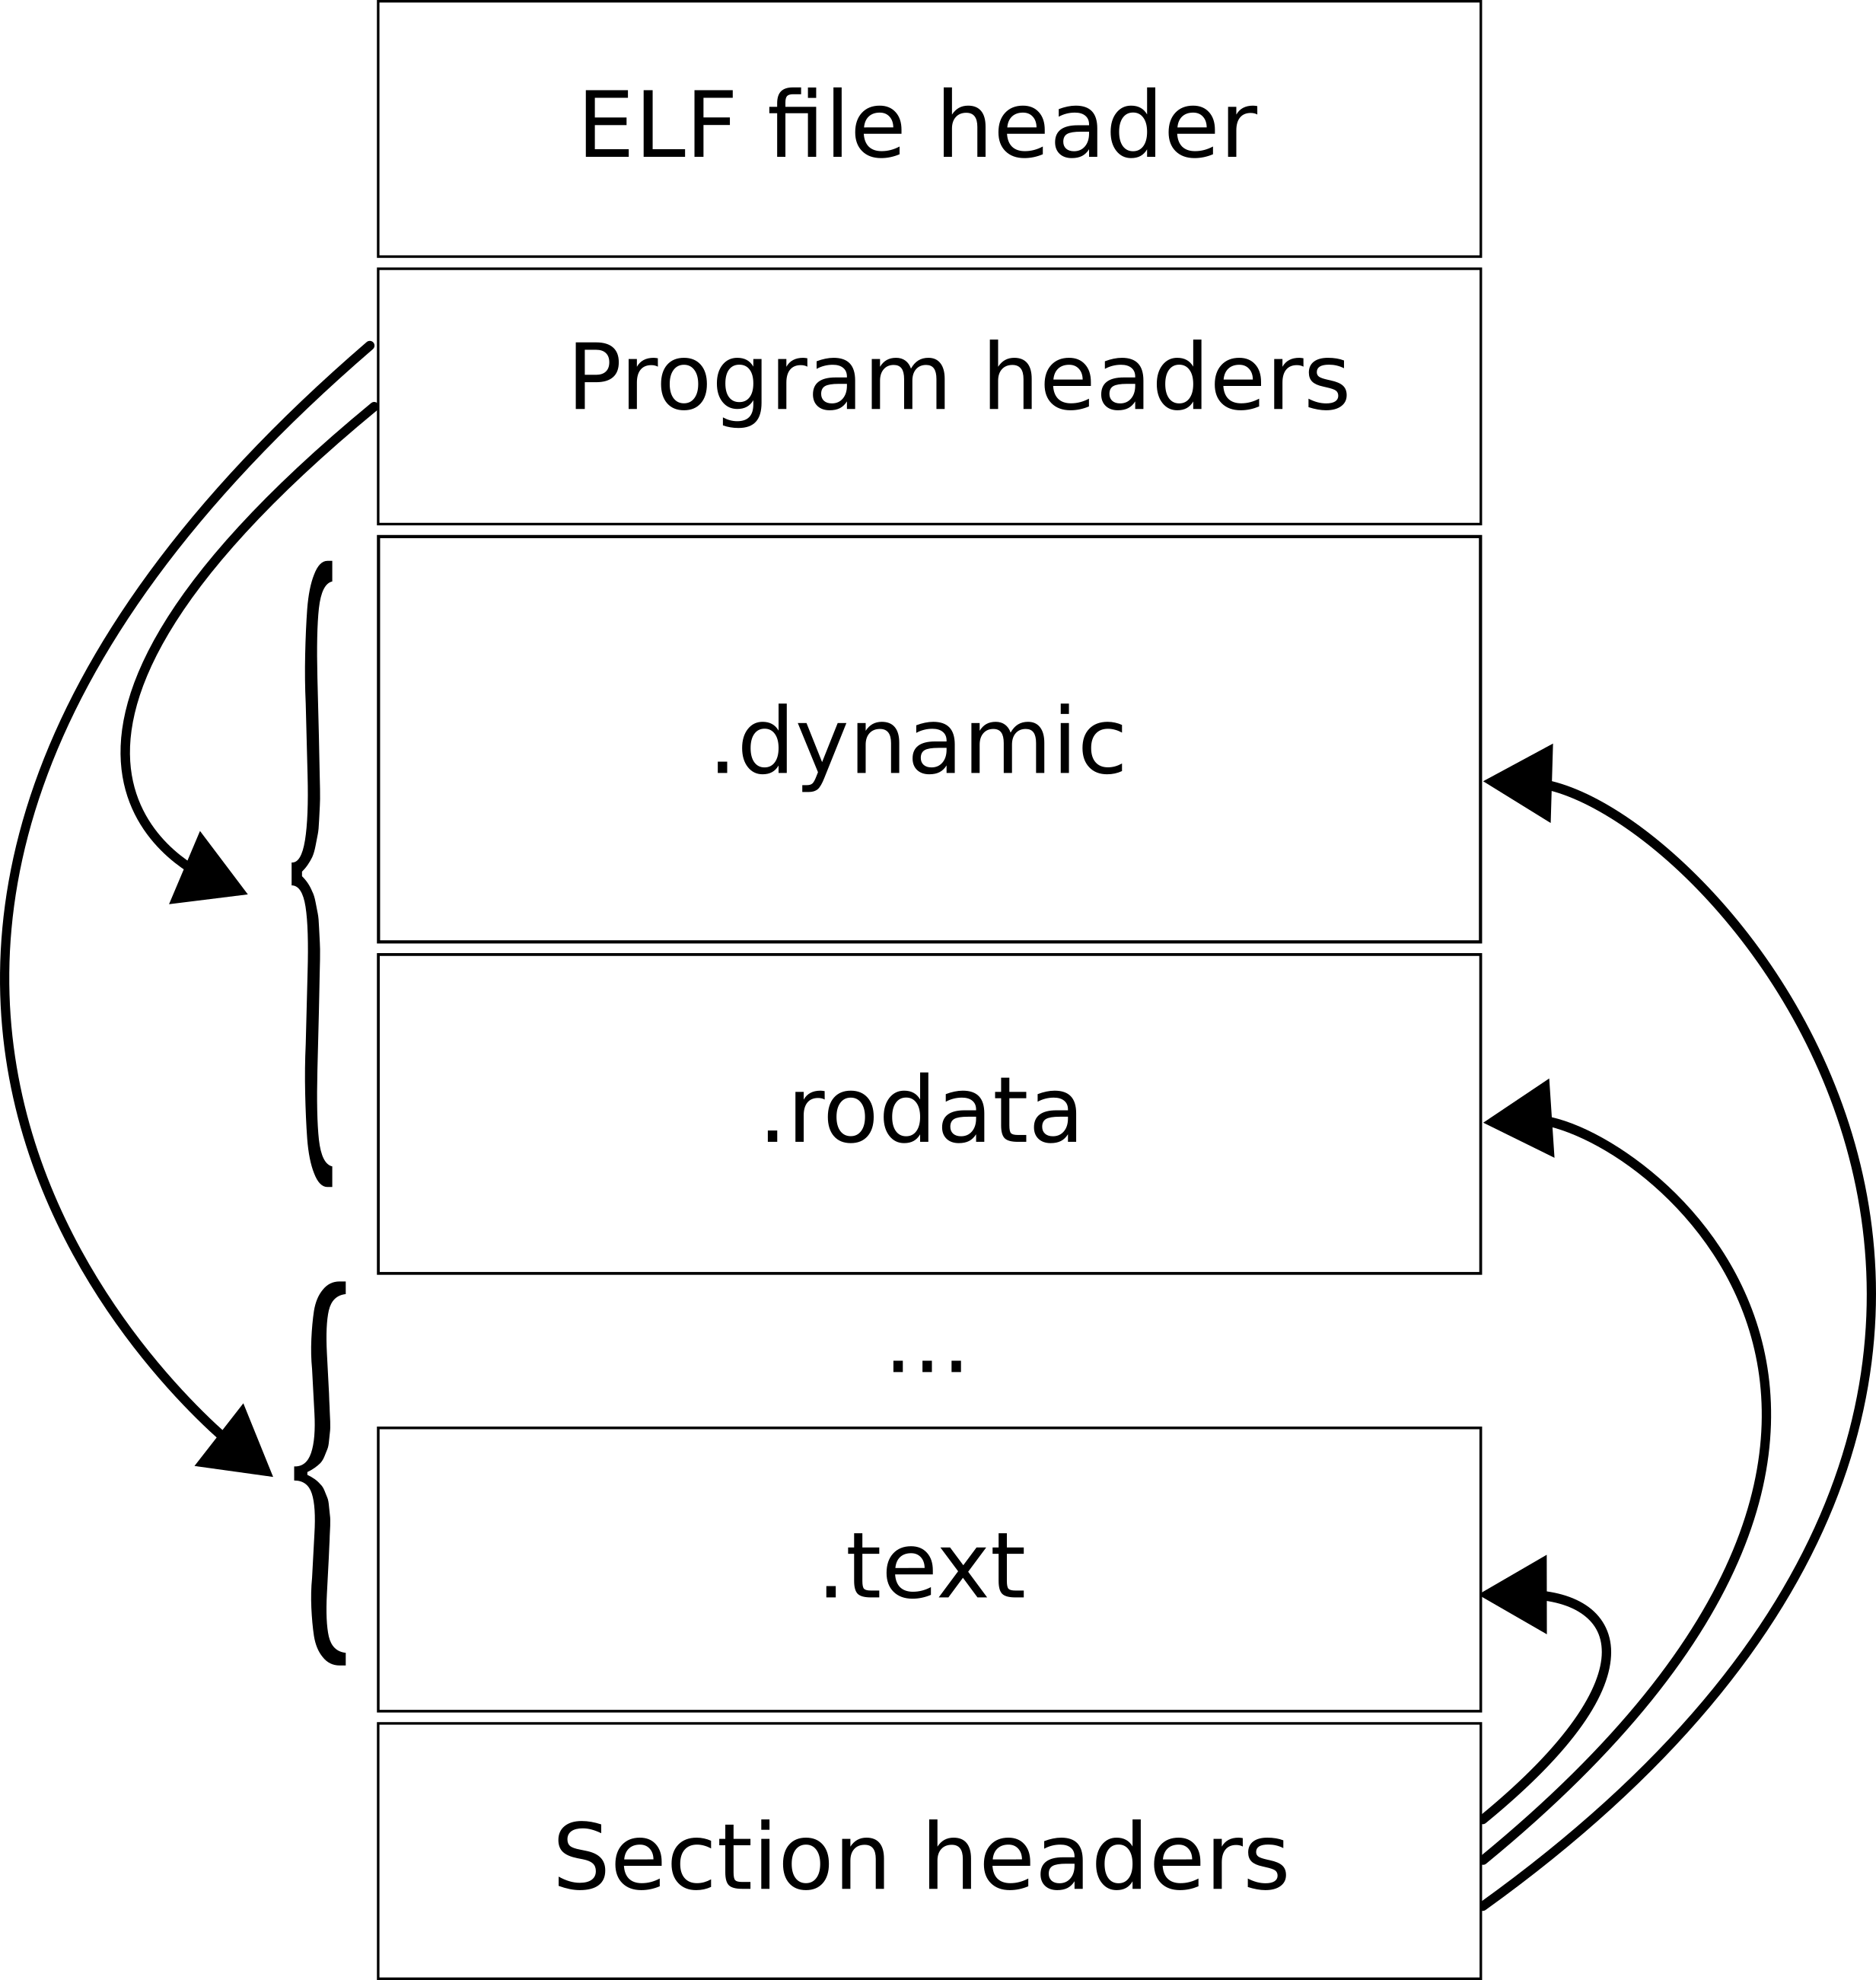
\includegraphics[width=0.5\textwidth]{inc/2_lit_review/elf_file_structure.png}
		\caption{The basic structure of an ELF file.\protect\footnotemark}
		\label{fig:elf_file_structure}
	\end{center}
\end{figure}
\footnotetext{Original image (CC BY-SA): \url{https://en.wikipedia.org/wiki/File:Elf-layout--en.svg}}

All ELF files starts with the four byte identifier \texttt{0x7F}, \texttt{'E'}, \texttt{'L'}, \texttt{'F'} which marks the beginning of the ELF file header. The ELF file header contains general information about a binary, such as its object file type (executable, relocatable or shared object), its assembly architecture (x86-64, ARM, …), the virtual address of its entry point which indicates the starting point of program execution, and the file offsets to the program and section headers.

Each program and section header describes a continuous segment or section of memory respectively. In general, segments are used by the linker to load executables into memory with correct access permissions, while sections are used by the compiler to categorize data and instructions. Therefore, the program headers are optional for relocatable and shared objects, while the section headers are optional for executables.

\begin{figure}[htbp]
	\begin{center}
		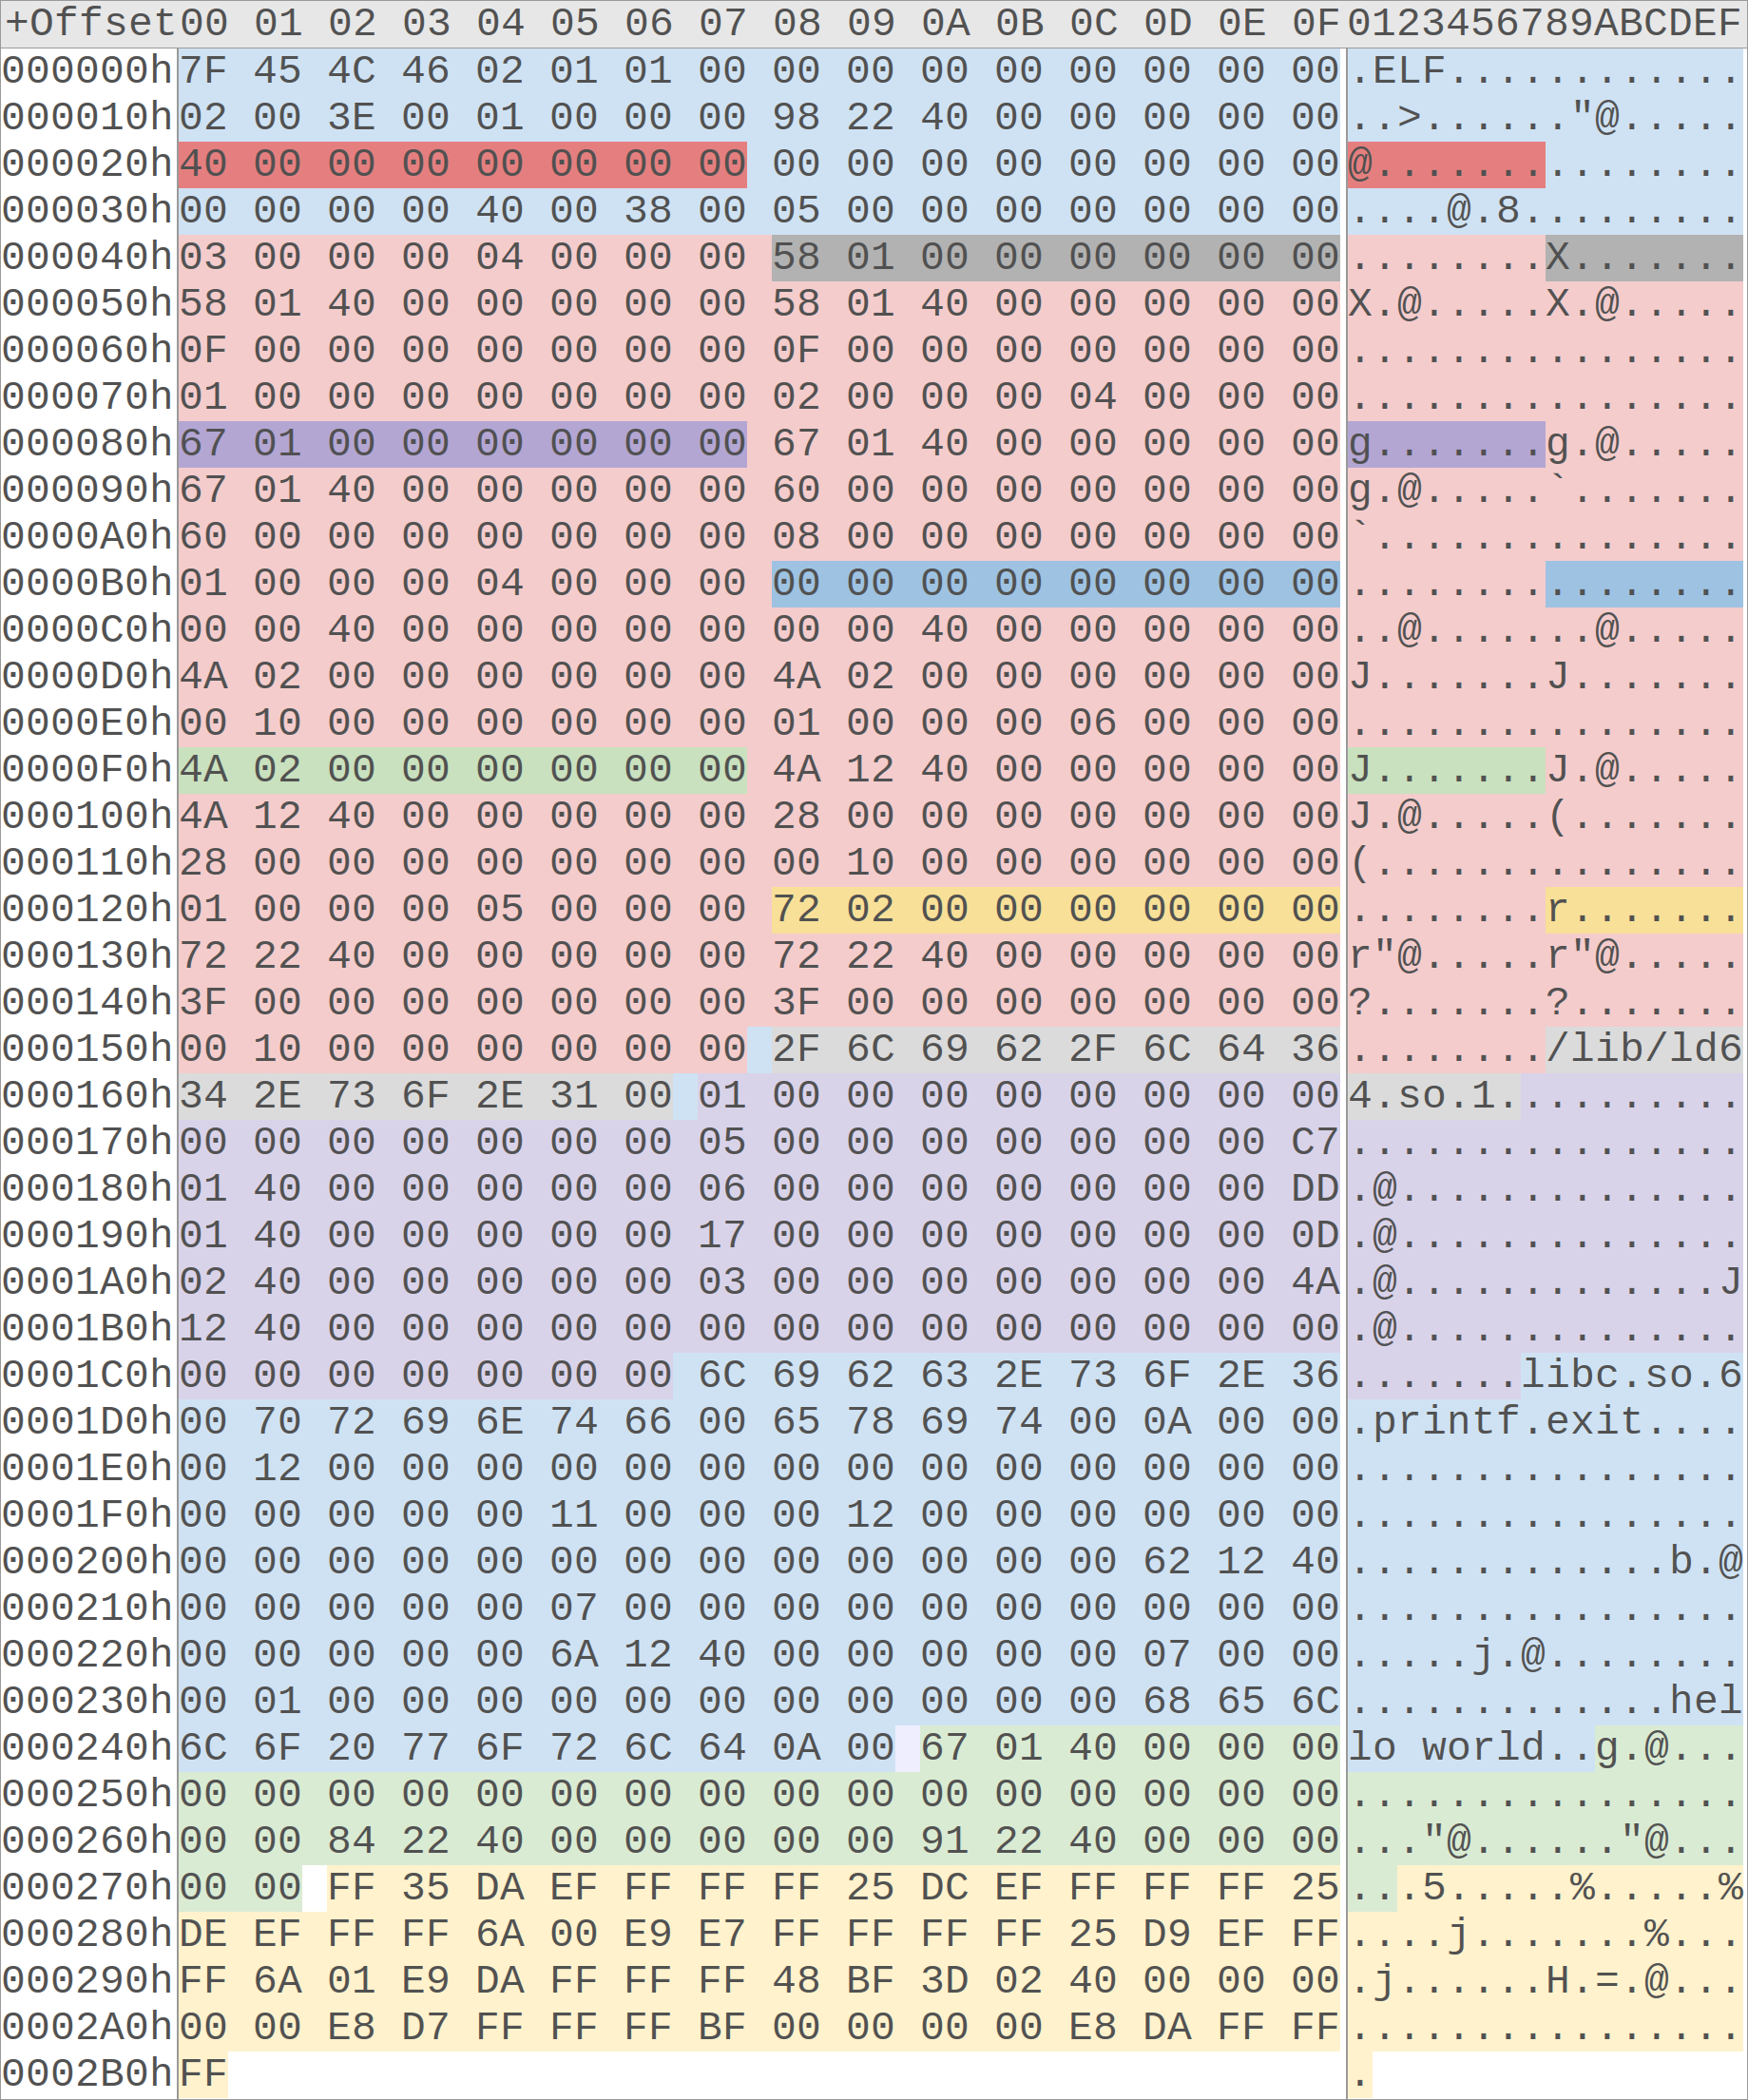
\includegraphics[width=\textwidth]{inc/2_lit_review/elf_dissection.png}
		\caption{The entire contents of a simple \textit{``hello world''} ELF executable with colour-coded file offsets, sections, segments and program headers. Each file offset is 8 bytes in width and coloured using a darker shade of its corresponding segment, section or program header.}
		\label{fig:elf_dissection}
	\end{center}
\end{figure}

To further investigate the structure of ELF files a simple 64-bit \textit{``hello world''} executable has been dissected and its content colour-coded. Each file offset of the executable consists of 8 bytes and is denoted in figure \ref{fig:elf_dissection} with a darker shade of the colour used by its corresponding target segment, section or program header. Starting at the middle of the ELF file header, at offset \texttt{0x20}, is the file offset (red) to the program table (bright red). The program table contains five program headers which specify the size and file offsets of two sections and three segments, namely the \texttt{.interp} (grey) and the \texttt{.dynamic} (purple) sections, and a \textit{read-only} (blue), a \textit{read-write} (green) and a \textit{read-execute} (yellow) segment.

Several sections are contained within the three segments. The \textit{read-only} segment contains the following sections:

\begin{itemize}
	\item \texttt{.interp}: the interpreter, i.e. the linker
	\item \texttt{.dynamic}: array of dynamic entities
	\item \texttt{.dynstr}: dynamic string table
	\item \texttt{.dynsym}: dynamic symbol table
	\item \texttt{.rela.plt}: relocation entities of the PLT
	\item \texttt{.rodata}: read-only data section
\end{itemize}

The \textit{read-write} segment contains the following section:

\begin{itemize}
	\item \texttt{.got.plt}: Global Offset Table (GOT) of the PLT (henceforth referred to as the GOT as this executable only contains one such table)
\end{itemize}

And the \textit{read-execute} segment contains the following sections:

\begin{itemize}
	\item \texttt{.plt}: Procedure Linkage Table (PLT)
	\item \texttt{.text}: executable code section
\end{itemize}

Seven of the nine sections contained within the executable are directly related to dynamic linking. The \texttt{.interp} section specifies the linker (in this case \textit{``/lib/ld64.so.1''}) and the \texttt{.dynamic} section an array of dynamic entities containing offsets and virtual addresses to relevant dynamic linking information. In this case the dynamic array specifies that \textit{``libc.so.6''} is a required library, and contains the virtual addresses to the \texttt{.dynstr}, \texttt{.dynsym}, \texttt{.rela.plt} and \texttt{.got.plt} sections. As noted, even a simple \textit{``hello world''} executable requires a large number of sections related to dynamic linking. Further analysis will reveal their relation to each other and describe their usage.

The dynamic string table contains the names of libraries (e.g. \textit{``libc.so.6''}) and identifiers (e.g. \textit{``printf''}) which are required for dynamic linking. Other sections refer to these strings using offsets into \texttt{.dynstr}. The dynamic symbol table declares an array of dynamic symbol entities, each specifying the name (e.g. offset to \textit{``printf''} in \texttt{.dynstr}) and binding information (local or global) of a dynamic symbol. Both the \texttt{.plt} and the \texttt{.rela.plt} sections refers to these dynamic symbols using array indicies. The \texttt{.rela.plt} section specifies the relocation entities of the PLT; more specifically this section informs the linker of the virtual address to the \texttt{.printf} and \texttt{.exit} entities in the GOT.

To reflect on how dynamic linking is accomplished on a Linux system lets review the assembly instructions of the executable \texttt{.text} and \texttt{.plt} sections as outlined in listing \ref{lst:elf_text} and \ref{lst:elf_plt} respectively.

\lstinputlisting[language=nasm, style=nasm, caption={The assembly instructions of the \texttt{.text} section. \label{lst:elf_text}}]{inc/2_lit_review/elf_text.asm}

\lstinputlisting[language=nasm, style=nasm, caption={The assembly instructions of the \texttt{.plt} section. \label{lst:elf_plt}}]{inc/2_lit_review/elf_plt.asm}

As visualised in listing \ref{lst:elf_text} the first call instruction of the \texttt{.text} section targets the \texttt{.printf} label of the \texttt{.plt} section instead of the actual address of the \textit{printf} function in the \textit{libc} library. The Procedure Linkage Table (PLT) provides a level of indirection between call instructions and actual function (procedure) addresses, and contains one entity per external function as outlined in listing \ref{lst:elf_plt}. The \texttt{.printf} entity of the PLT contains a jump instruction which targets the address stored in the \texttt{.printf} entity of the GOT. Initially this address points to the next instruction, i.e. the instruction denoted by the \texttt{.resolve\_printf} label in the PLT. On the first invokation of \textit{printf} the linker replaces this address with the actual address of the \textit{printf} function in the \textit{libc} library, and any subsequent invokation of \textit{printf} will target the resolved function address directly.

This method of external function resolution is called lazy dynamic linking as it postpones the work and only resolves a function once it is actually invoked at runtime. The lazy approach to dynamic linking may improve performance by limiting the number of symbols that require resolution. At the same time the eager approach may benefit latency sensitive applications which cannot afford the cost of dynamic linking at runtime.

A closer look at the instructions denoted by the \texttt{.resolve\_printf} label in listing \ref{lst:elf_plt} reveals how the linker knows which function to resolve. Essentially the \textit{dl\_runtime\_resolve} function is invoked with two arguments, namely the dynamic symbol index of the \textit{printf} function and a pointer to a linked list of nodes, each refering to the \texttt{.dynamic} section of a shared object. Upon termination the linked list of our \textit{``hello world''} process contains a total of four nodes, one for the executable itself and three for its dynamically loaded libraries, namely \textit{linux-vdso.so.1}, \textit{libc.so.6} and \textit{ld64.so.1}.

To summarise, the execution of a dynamically linked executable can roughly be described as follows. Upon execution the kernel parses the program headers of the ELF file, maps each segment to one or more pages in memory with appropriate access permissions, and transfers the control of execution to the linker (\textit{``/lib/ld64.so.1''}) which was loaded in a similar fashion. The linker is responsible for initiating the addresses of the \textit{dl\_runtime\_resolve} function and the aforementioned linked list, both of which are stored in the GOT of the executable. After this setup is complete the linker transfers control to the entry point of the executable, as specified by the ELF file header (in this case the \texttt{.start} label of the \texttt{.text} section). At this point the assembly instructions of the application are executed until termination and external functions are lazily resolved at runtime by the linker through invocations to the \textit{dl\_runtime\_resolve} function.

% --- [ Decompilation Phases ] -------------------------------------------------

\subsection{Decompilation Phases}
\label{sec:lit_review_decompilation_phases}

A core principle utilized in decompilers is the separation of concern through the use of abstractions, and extensive work involves translating into and breaking out of various abstraction layers. In general, a decompiler is composed of distinct phases which parse, analyse or transform the input. These phases are conceptually grouped into three modules to separate concerns regarding source machine language and target programming language. Firstly, the front-end module parses executable files and translates their platform-dependent assembly into a platform-independent intermediate representation (IR). Secondly, the middle-end module performs a set of decompilation passes to lift the IR, from a low-level to a high-level representation, by reconstructing high-level control structures and expressions. Lastly, the back-end module translates the high-level IR to a specific target programming language \cite{reverse_comp}. Figure \ref{fig:modules_overview} gives an overview of the decompilation modules and visualises their relationship.

\begin{figure}[htbp]
	\begin{center}
		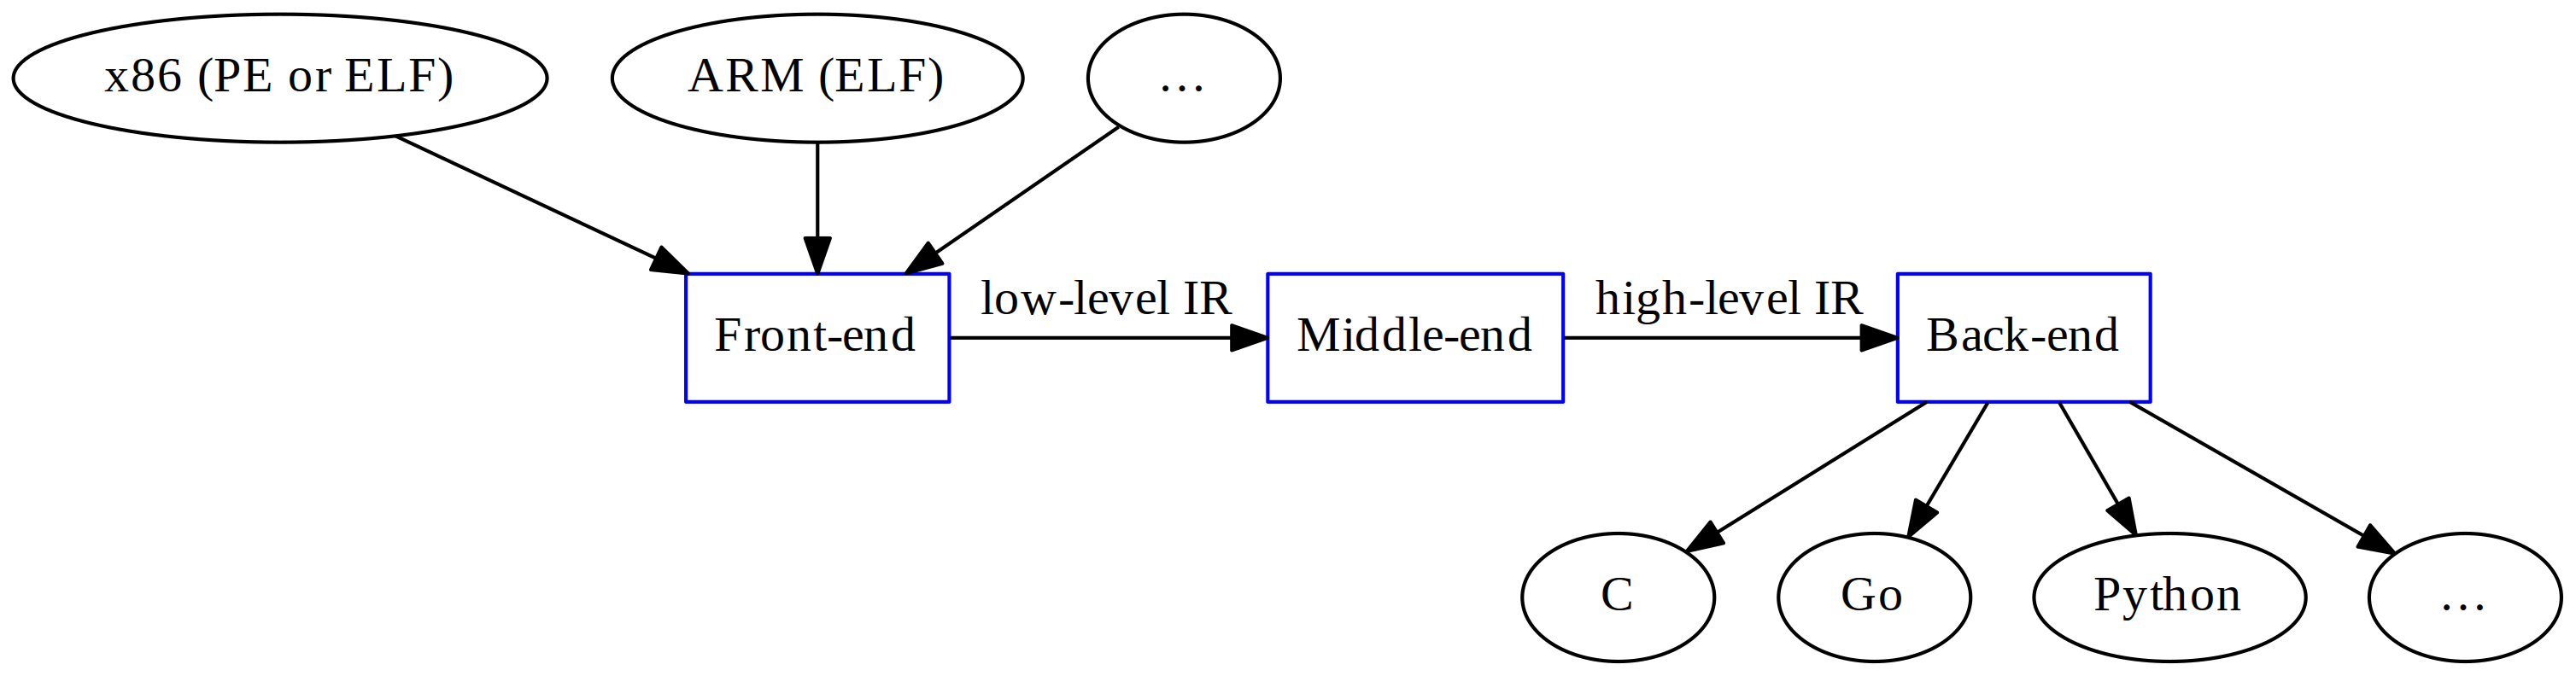
\includegraphics[width=\textwidth]{inc/2_lit_review/modules_overview.png}
		\caption{Firstly, the front-end module accepts several executable file formats (PE, ELF, …) as input and translates their platform-dependent assembly (x86, ARM, …) to a low-level IR. Secondly, the middle-end module lifts the low-level IR to a high-level IR through a set of decompilation passes. Lastly, the back-end module translates the high-level IR into one of several target programming languages (C, Go, Python, …).}
		\label{fig:modules_overview}
	\end{center}
\end{figure}

The remainder of this section describes the distinct decompilation phases, most of which have been thoroughly described by Cristina Cifuentes in her influential paper \textit{``Reverse Compilation Techniques''} \cite{reverse_comp}.

% --- [ Subsubsections ] -------------------------------------------------------

% ~~~ [ Binary Analysis ] ~~~~~~~~~~~~~~~~~~~~~~~~~~~~~~~~~~~~~~~~~~~~~~~~~~~~~~

\subsubsection{Binary Analysis}
\label{sec:lit_review_binary_analysis}

As demonstrated in section \ref{sec:lit_review_the_anatomy_of_an_executable}, parsing even a simple \textit{``hello world''} executable requires extensive knowledge of its binary file format (in this case ELF). The binary analysis phase is responsible for parsing input files of various binary file formats, such as PE and ELF, and present their content in a uniform manner which preserves the relations between file contents, virtual addresses and access permissions. Later stages of the decompilation pipeline builds upon this abstraction to access the file contents of each segment or section without worrying about the details of the underlying file format. Information about external symbols, metadata and the computer architecture of the assembly may also be provided by this abstraction.

% ~~~ [ Disassembly ] ~~~~~~~~~~~~~~~~~~~~~~~~~~~~~~~~~~~~~~~~~~~~~~~~~~~~~~~~~~

\subsubsection{Disassembly}

The disassembly phase (referred to as the \textit{syntactic analysis phase} by C. Cifuentes) is responsible for decoding the raw machine instructions of the executable segments into assembly. The computer architecture dictates how the assembly instructions and their associated operands are encoded. Generally CISC architectures (e.g. x86) use variable length instruction encoding (e.g. instructions occupy between 1 and 17 bytes in x86) and allow memory addressing modes for most instructions (e.g. arithmetic instructions may refer to memory locations in x86) \cite{x86_manual}. In contract, RISC architectures (e.g. ARM) generally use fixed-length instruction encoding (e.g. instructions always occupy 4 bytes in AArch64) and only allow memory access through load-store instructions (e.g. arithmetic instructions may only refer to registers or immediate values in ARM) \cite{arm_manual}.

One of the main problems of the disassembly phase is how to separate code from data. In the Von Neumann architecture the same memory unit may contain both code and data. Furthermore, the data stored in a given memory location may be interpreted as code by one part of the program, and as data by another part. In contrast, the Harvard architecture uses separate memory units for code and data \cite{von_neumann_vs_harvard}. Since the use of the Von Neumann architecture is wide spread, solving this problem is fundamental for successful disassemblers.

% TODO: Add switch tables example.

A solution to the problem of separating code from data is to use recursive descent instead of linear descent when parsing assembly instructions.

% TODO: Add description of recursive descent and linear descent.

\begin{figure}[htbp]
	\centering
	\begin{subfigure}[t]{0.49\textwidth}
		\lstinputlisting[language=nasm, style=nasm, tabsize=2]{inc/hello/hello_linear.asm}
		\caption{Disassembly from \texttt{objdump} and \texttt{ndisasm}\protect\footnotemark.}
	\end{subfigure}
	\qquad
	\begin{subfigure}[t]{0.35\textwidth}
		\lstinputlisting[language=nasm, style=nasm, tabsize=2]{inc/hello/hello_recursive.asm}
		\caption{Disassembly from IDA Pro.}
	\end{subfigure}
	\caption{The disassembly produced by a linear descent parser (left) and a recursive descent parser (right) when analyzing a simple \textit{``hello world''} program that stores the \texttt{hello} string in the executable segment.}
\end{figure}
\footnotetext{The Netwide Disassembler: \url{http://www.nasm.us/doc/nasmdoca.html}}

One problem faced by both linear descent and recursive descent disassemblers is the need for a starting point. In practise, exported entry point symbols (e.g. \texttt{main}, \texttt{start}, \texttt{DLLMain}, …) works well.

% TODO: Verify that it is called symbolic execution/symbolic execution engine.

Another problem for recursive descent disassemblers is indirect branches (e.g. jump to the address stored in a register). In the case of indirect branches, it is impossible to know the branch target by only looking at the individual instructions. One solution is to use symbolic execution, which emulates the processor and executes instructions to give information about the value stored in registers. With this method the target of indirect jumps may be calculated. There are problems to consider when designing a symbolic execution engine, for instance the impact of cached memory access. See figure \ref{foo} for an example of where cache details matter for the execution flow.

% TODO: Add example where the cache impacts execution flow (pipeline pre-schedules). *addr = 5; jmp addr

% Problems:
% * self-modifying code
% * Architecture-dependent Restrictions
%    Cannot be determined by step-by-step debugging; as the prefetch pipeline
%    would behave differently.
%       mov ax, 0x9090
%       mov [jmpDef], ax
%    jmpDef:
%       jmp codeExecuted
%    codeNotExecuted:
%       foo
%    codeExecuted:
%       bar

Another issue is the use of callbacks, which is common in GUI applications.
% TODO: Solution? Run program and use breakpoints?

There exists several anti-disassembly techniques which are commonly used by malware. One such technique exploits the fact that recursive descent parsers follow both the true and the false branch of conditional branch instructions, as demonstrated in figure \ref{fig:anti-disassembly}.

The recursive descent parser cannot parse both the false and the true-branch of the conditional branch instruction at line 3, because the true branch targets the middle of a \texttt{jmp} instruction.

The conditional branch instruction at line 3 always takes the true branch, which points to the middle of the \texttt{jmp} instruction decoded when parsing the false branch. The recursive descent parser cannot disassembly both branches and is forced to choose one of them, in this case the \texttt{fake} branch.

The recursive descent parser fails by using a conditional branch instruction (\texttt{jz}) which always takes the true-branches \texttt{fake+1} which is in the middle of an instruction.

\begin{figure}[htbp]
	\centering
	\begin{subfigure}[t]{0.59\textwidth}
		\lstinputlisting[language=nasm, style=nasm, tabsize=2]{inc/hello/anti_orig.asm}
		\caption{Original assembly.}
	\end{subfigure}
	\qquad
	\begin{subfigure}[t]{0.34\textwidth}
		\lstinputlisting[language=nasm, style=nasm, tabsize=2]{inc/hello/anti_fail.asm}
		\caption{Disassembly from IDA Pro.}
	\end{subfigure}
	\caption{The original assembly (left) contains an anti-disassembly trick which causes the recursive descent parser to fail (right).}
	\label{fig:anti-disassembly}
\end{figure}

The anti-disassembly technique presented in figure \ref{fig:anti-disassembly} may be mitigated using symbolic execution, which could verify that the conditional jump always takes the true branch and therefore allow the instruction to be replaced with an unconditional jump to the target of the true branch. This quickly becomes a game of cat-and-mouse, as the anti-disassembly techniques could be extended to rely on network activity, file contents, or other external sources which would render the symbolic exeuction useless.

To conclude, the disassembly phase deals with non-trivial problems, some of which are difficult to automate. Advanced disassemblers therefore provide interactive capabilities and rely on human intuition to solve ambiguities and direct the disassembler out of corner cases. See section \ref{sec:related_work_hex-rays_decompiler} for further details on such disassemblers.

% TODO: Introduce the various approaches and highlight their individual
% strengths and weaknesses.
%
% NAIVE APPROACH: linear descent disassemblers.
% PROBLEM: Highlight problems with linear descent disassemblers.
%    - rodata (e.g. "hello world") and jump tables in code.
%
% SOLUTION: recursive descent disassemblers.
% PROBLEM: Highlight problems with recursive descent disassemblers.
%    - Distinguish between code and data (e.g. find entry points of functions).
%      Not add functions are directly referred to (e.g. callback functions which
%      are commonly used by GUI applications).
%    - Easy to fool.
%       xor eax, eax
%       cmp eax, 0
%       jz foo+1 ; Cannot disassembly both foo and foo+1.
% foo:
%       add eax, 3
%
% SOLUTION: symbolic execution engines.
% PROBLEM: security, performance, ...?

% ~~~ [ Control Flow Analysis ] ~~~~~~~~~~~~~~~~~~~~~~~~~~~~~~~~~~~~~~~~~~~~~~~~

\subsubsection{Control Flow Analysis}
\label{sec:lit_review_control_flow_analysis}

The control flow analysis stage is responsible for analysing the control flow (i.e. flow of execution) of source programs to recover their high-level control flow structures. The control flow of a given function is determined by its branching instructions and may be expressed as a control flow graph (CFG), which is a connected graph with a single entry node (the function entry point) and zero or more exit nodes (the function return statements). A key insight provided by C. Cifuentes and S. Moll is that high-level control flow primitives (such as 1-way conditionals and pre-test loops) may be expressed using graph representations \cite{reverse_comp, decomp_of_llvm}, as illustrated in figure \ref{fig:graph_representations}. The problem of recovering high-level control flow primitives from CFGs may therefore be reformulated as the problem of identifying subgraphs (i.e. the graph representation of a high-level control flow primitive) in graphs (i.e. the CFG of a function) without considering node names. This problem is commonly referred to as \textit{subgraph isomorphism search}, the general problem of which is NP-hard \cite{subgraph_isomorphism_algorithms}. However, the problem which is required to be solved by the control flow analysis stage may be simplified by exploiting known properties of CFGs (e.g. connected graph with a single entry node).

\begin{figure}[htbp]
	\centering
	% if
	\begin{subfigure}[ht]{0.23\textwidth}
		\centering
		\begin{subfigure}[ht]{0.45\textwidth}
			\lstinputlisting[language=go, style=go, breaklines=false, numbers=none]{inc/primitives/if.c}
		\end{subfigure}
		\begin{subfigure}[ht]{0.42\textwidth}
			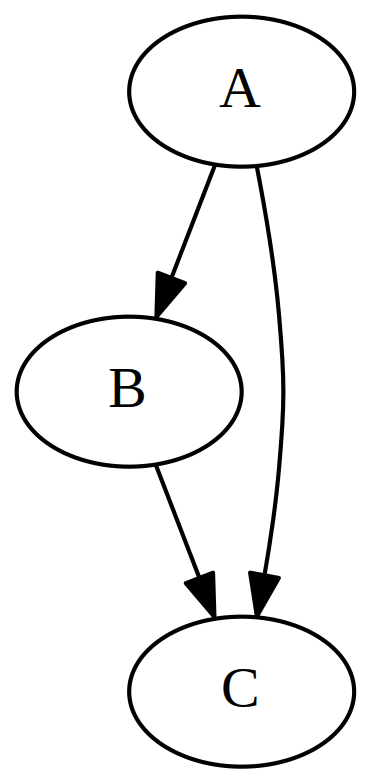
\includegraphics[width=\textwidth]{inc/primitives/if.png}
		\end{subfigure}
		\caption{1-way conditional; entry: \texttt{A}, exit: \texttt{C}.}
		\label{fig:if_graph_representation}
	\end{subfigure}
	\qquad
	% if_else
	\begin{subfigure}[ht]{0.28\textwidth}
		\centering
		\begin{subfigure}[ht]{0.45\textwidth}
			\lstinputlisting[language=go, style=go, breaklines=false, numbers=none]{inc/primitives/if_else.c}
		\end{subfigure}
		\begin{subfigure}[ht]{0.50\textwidth}
			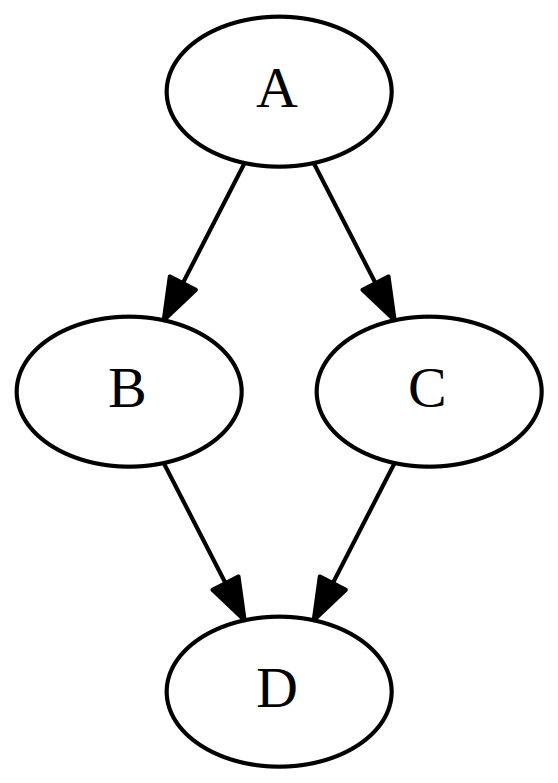
\includegraphics[width=\textwidth]{inc/primitives/if_else.png}
		\end{subfigure}
		\caption{2-way conditional; entry: \texttt{A}, exit: \texttt{D}.}
		\label{fig:if_else_graph_representation}
	\end{subfigure}
	\qquad
	% if_return
	\begin{subfigure}[ht]{0.30\textwidth}
		\centering
		\begin{subfigure}[ht]{0.45\textwidth}
			\lstinputlisting[language=go, style=go, breaklines=false, numbers=none]{inc/primitives/if_return.c}
		\end{subfigure}
		\begin{subfigure}[ht]{0.50\textwidth}
			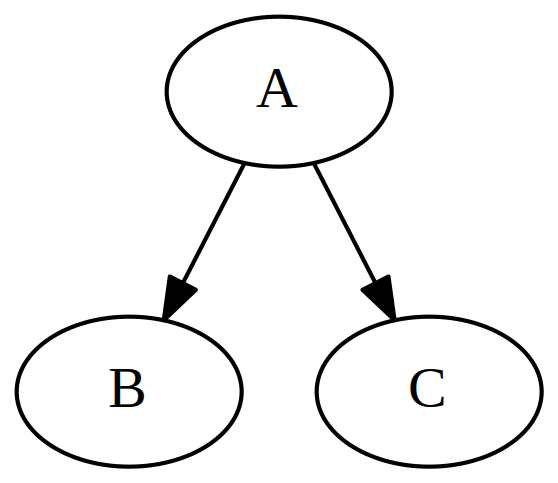
\includegraphics[width=\textwidth]{inc/primitives/if_return.png}
		\end{subfigure}
		\caption{1-way condition with return statement in body; entry: \texttt{A}, exit: \texttt{C}.}
		\label{fig:if_return_graph_representation}
	\end{subfigure}
	\qquad
	% pre_loop
	\begin{subfigure}[ht]{0.32\textwidth}
		\centering
		\begin{subfigure}[ht]{0.45\textwidth}
			\lstinputlisting[language=C, style=go, breaklines=false, numbers=none]{inc/primitives/pre_loop.c}
		\end{subfigure}
		\begin{subfigure}[ht]{0.50\textwidth}
			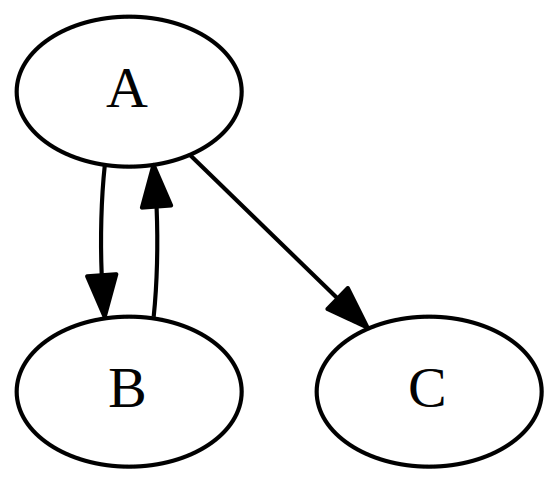
\includegraphics[width=\textwidth]{inc/primitives/pre_loop.png}
		\end{subfigure}
		\caption{pre-test loop; entry: \texttt{A}, exit: \texttt{C}.}
		\label{fig:pre_loop_graph_representation}
	\end{subfigure}
	\qquad
	% post_loop
	\begin{subfigure}[ht]{0.30\textwidth}
		\centering
		\begin{subfigure}[ht]{0.50\textwidth}
			\lstinputlisting[language=C, style=go, breaklines=false, numbers=none]{inc/primitives/post_loop.c}
		\end{subfigure}
		\begin{subfigure}[ht]{0.35\textwidth}
			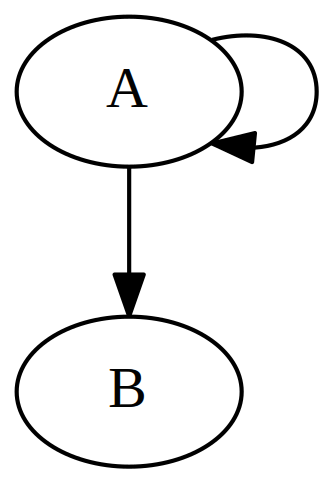
\includegraphics[width=\textwidth]{inc/primitives/post_loop.png}
		\end{subfigure}
		\caption{post-test loop; entry: \texttt{A}, exit: \texttt{B}.}
		\label{fig:post_loop_graph_representation}
	\end{subfigure}
	\qquad
	% list
	\begin{subfigure}[ht]{0.24\textwidth}
		\centering
		\begin{subfigure}[ht]{0.20\textwidth}
			\lstinputlisting[language=C, style=go, breaklines=false, numbers=none]{inc/primitives/list.c}
		\end{subfigure}
		\begin{subfigure}[ht]{0.35\textwidth}
			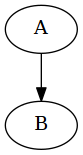
\includegraphics[width=\textwidth]{inc/primitives/list.png}
		\end{subfigure}
		\caption{consecutive statements; entry: \texttt{A}, exit: \texttt{B}.}
		\label{fig:list_graph_representation}
	\end{subfigure}
	\caption{The pseudo-code and graph representation of various high-level control flow primitives with denoted entry and exit nodes.}
	\label{fig:graph_representations}
\end{figure}

When the subgraph isomorphism of a high-level control flow primitive has been identified in the CFG of a function, it may be replaced by a single node that inherits the predecessors of the subgraph entry node and the successors of the subgraph exit node; as illustrated in figure \ref{fig:subgraph_merge}. By recording the node names of the identified subgraphs and the name of their corresponding high-level control flow primitives, the high-level control flow structure of a CFG may be recovered by successively identifying subgraph isomorphisms and replacing them with single nodes until the entire CFG has been reduced into a single node; as demonstrated by the step-by-step simplification of a CFG in appendix \ref{app:control_flow_analysis_example}. Should the control flow analysis fail to reduce a CFG into a single node, the CFG is considered irreducible with regards to the supported high-level control flow primitives (see figure \ref{fig:graph_representations}). To structure arbitrary irreducible graphs, S. Moll applied node splitting (which translates irreducible graphs into reducible graphs by duplicating nodes) to produce functionally equivalent target programs \cite{decomp_of_llvm}. In contrast, C. Cifuentes focused on preserving the structural semantics of the source program (which may be required in forensics investigations), and therefore used \texttt{goto}-statements in these cases to produce unstructured target programs.

\begin{figure}[htbp]
	\centering
	\begin{subfigure}[ht]{0.15\textwidth}
		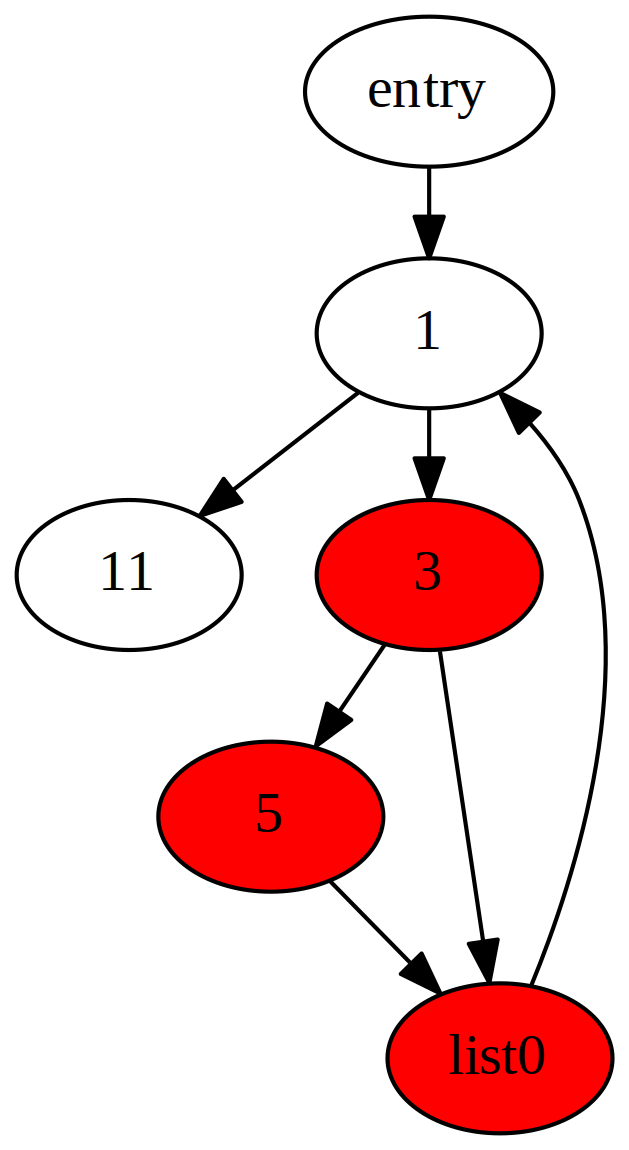
\includegraphics[width=\textwidth]{inc/2_lit_review/cfg_pre_merge.png}
	\end{subfigure}
	\qquad
	\begin{subfigure}[ht]{0.15\textwidth}
		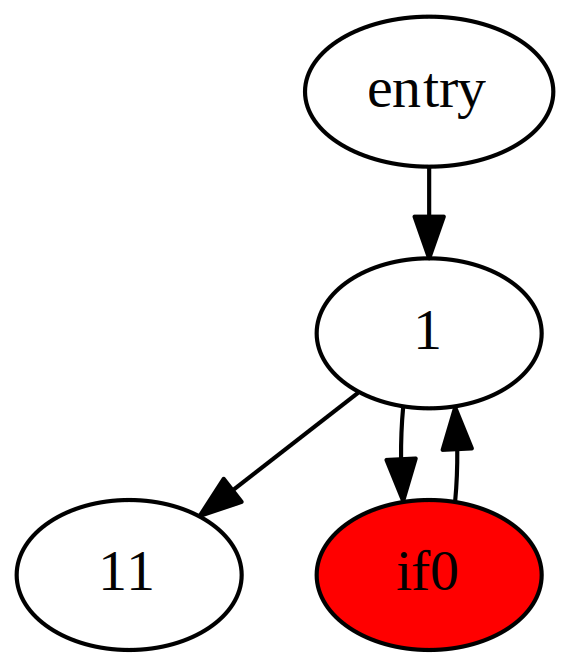
\includegraphics[width=\textwidth]{inc/2_lit_review/cfg_post_merge.png}
	\end{subfigure}
	\caption{The left side illustrates the CFG of a function in which the graph representation of a 1-way conditional (see figure \ref{fig:if_graph_representation}) has been identified, and the right side illustrates the same CFG after the subgraph has been replaced with a single node (i.e. \texttt{if0}) that inherits the predecessors of the subgraph entry node (i.e. \texttt{3}) and the successors of the subgraph exit node (i.e. \texttt{list0}).}
	\label{fig:subgraph_merge}
\end{figure}


% --- [ Evaluation of Intermediate Representations ] ---------------------------

\subsection{Evaluation of Intermediate Representations}

Decompilers face similar problems as both binary analysis tools and compilers. Therefore, it seems reasonable that the intermediate representations (IRs) used in these domains may be well suited for decompilation purposes. This section evaluates one IR from each domain with regards to their suitability for recovering high-level control flow primitives (objective \ref{itm:obj_control_flow_analysis_component}) and expressions (objective \ref{itm:obj_data_analysis_library}).

% ~~~ [ REIL ] ~~~~~~~~~~~~~~~~~~~~~~~~~~~~~~~~~~~~~~~~~~~~~~~~~~~~~~~~~~~~~~~~~

\subsubsection{REIL}

The Reverse Engineering Intermediate Language (REIL) is a very simple and platform independent assembly language. The REIL instruction set contains only 17 different instructions, each with exactly three (possibly empty) operands. The first two operands are always used for input and the third for output (except for the conditional jump instruction which uses the third operand as the jump target). Furthermore, each instruction has at most one effect on the global state and never any side-effects (such as setting flags) \cite{reil_paper,reil_spec}. Thanks to the simplicity of REIL a full definition of its instruction set has been provided in appendix \ref{app:reil_instructions}, which includes examples of each instruction and defines their syntax and semantics (in pseudo C-code).

When translating native assembly (e.g. x86) into REIL, the original addresses of each instruction is left shifted by 8 bits to allow 256 REIL instructions per address. Each native instruction may therefore be translated into one or more REIL instructions (at most 256), which is required to correctly map the semantics of complex instructions with side-effects. This systematic approach of deriving instruction addresses has a fundamental implication, REIL supports indirect branches (e.g. \texttt{call rax}) by design.

The language was originally designed to assist static code analysis and translators from native assembly (x86, PowerPC-32 and ARM-32) to REIL are commercially available. However, the project home page has not been updated since Google acquired zynamics in 2011. Since then approximately 10 papers have been published which references REIL and the adaptation of the language within the open source community seems limited. As of 2015-01-04 only three implementations existed on GitHub (two in Python\footnote{Binary Analysis and RE Framework: \url{https://github.com/programa-stic/barf-project}}\footnote{REIL translation library: \url{https://github.com/c01db33f/pyreil}} and one in C\footnote{Binary introspection toolkit: \url{https://github.com/aoikonomopoulos/bit}}), and the most popular had less than 25 watchers, 80 stars and 15 forks.

A fourth implementation was released at the 15th of March 2015 however, and in less than two weeks OpenREIL had become the most popular REIL implementation on GitHub. The OpenREIL project extends the original REIL instruction set with signed versions of the multiplication, division and modulo instructions, and includes convenience instructions for common comparison and binary operations. OpenREIL is currently capable of translating x86 executables to REIL, and aims to include support for ARM and x86-64 in the future. Furthermore, the OpenREIL project intends to implement support for translating REIL to LLVM IR, thus bridging the two intermediate representations \cite{openreil}.

% ~~~ [ LLVM IR ] ~~~~~~~~~~~~~~~~~~~~~~~~~~~~~~~~~~~~~~~~~~~~~~~~~~~~~~~~~~~~~~

\subsubsection{LLVM IR}
\label{sec:lit_review_llvm_ir}

The LLVM compiler framework defines an intermediate representation called LLVM IR, which works as a language-agnostic and platform-independent bridge between high-level programming languages and low-level machine architectures. The majority of the optimizations of the LLVM compiler framework target LLVM IR, thus separating concerns related to the source language and target architecture \cite{llvm_architecture}.

There exist three isomorphic forms of LLVM IR; a human-readable assembly representation, an in-memory data structure, and an efficient binary bitcode file format. Several tools are provided by the LLVM compiler framework to convert LLVM IR between the various representations. The LLVM IR instruction set is comparable in size to the MIPS instruction set, and both uses a load/store architecture \cite{mips_ref,llvm_lang_ref}.

Function definitions in LLVM IR consist of a set of basic blocks. A basic block is a sequence of zero or more non-branching instructions (e.g. \texttt{add}), followed by a terminating instruction (i.e. a branching instruction; e.g. \texttt{br}, \texttt{ret}). The key idea behind a basic block is that if one instruction of the basic block is executed, all instructions are executed. This concept vastly simplifies control flow analysis as multiple instructions may be regarded as a single unit \cite{decomp_of_llvm}.

LLVM IR is represented in Static Single Assignment (SSA) form, which guarantees that every variable is assigned exactly once, and that every variable is defined before being used. These properties simplifies a range of optimizations (e.g. constant propagation, dead code elimination). For the same reasons, the Boomerang decompiler uses an IR in SSA form to simplify expression propagation \cite{ssa_for_decomp}.

In recent years other research groups have started developing decompilers \cite{decomp_of_llvm,retargetable_decomp} and reverse engineering components \cite{mcsema} which rely on LLVM IR. There may exist an IR which is more suitable in theory, but in practice the collaboration and reuse of others efforts made possible by the vibrant LLVM community is a strong merit in and of itself.

To conclude the evaluation, LLVM IR has been deemed suitable for the decompilation pipeline. The middle-end of the decompilation pipeline requires an IR which provides a clear separation between low-level machine architectures and high-level programming languages, and LLVM IR was designed with the same requirements in mind. Furthermore, the wide range of tools and optimizations provided by the LLVM compiler framework may facilitate decompilation workflows. The control flow analysis (see section \ref{sec:lit_review_control_flow_analysis}) of the decompilation pipeline will benefit from the notion of basic blocks in LLVM IR. Similarly, the data flow analysis will benefit from the SSA form of LLVM IR.


